% Hlavicka pro protokoly z fyzikalniho praktika.
% Verze pro: LaTeX
% Verze hlavicky: 22. 2. 2007
% Autor: Ustav fyziky kondenzovanych latek
% Ke stazeni: www.physics.muni.cz/ufkl/Vyuka/
% Licence: volne k pouziti, nejlepe k vcasnemu odevzdani protokolu z Vaseho mereni.


\documentclass[czech,11pt,a4paper]{article}
\usepackage[T1]{fontenc}
\usepackage{graphicx}
\usepackage{mathtools}
\usepackage{amssymb}
\usepackage{amsthm}
\usepackage{thmtools}
\usepackage{xcolor}
\usepackage{nameref}
\usepackage{babel}
\usepackage{hyperref}
\usepackage{multicol}
\usepackage[export]{adjustbox}
\usepackage{subcaption}
\usepackage{caption}
\usepackage{multirow}
\usepackage{float}
\usepackage{placeins}


%%% Nemente:
\usepackage[margin=2cm]{geometry}
\newtoks\jmenopraktika \newtoks\jmeno \newtoks\datum
\newtoks\obor \newtoks\skupina \newtoks\rocnik \newtoks\semestr
\newtoks\cisloulohy \newtoks\jmenoulohy
\newtoks\tlak \newtoks\teplota \newtoks\vlhkost
%%% Nemente - konec.


%%%%%%%%%%% Doplnte pozadovane polozky:

\jmenopraktika={Fyzikální praktikum 1}  % nahradte jmenem vaseho predmetu
\jmeno={Teodor Duraković}            % nahradte jmenem mericiho
\datum={27.~března 2024}        % nahradte datem mereni ulohy
\obor={F}                     % nahradte zkratkou vami studovaneho oboru
\skupina={St 8:00}            % nahradte dobou vyuky vasi seminarni skupiny
\rocnik={I}                  % nahradte rocnikem, ve kterem studujete
\semestr={II}                 % nahradte semestrem, ve kterem studujete

\cisloulohy={1}               % nahradte cislem merene ulohy
\jmenoulohy={Měření teploty} % nahradte jmenem merene ulohy

\tlak={98 \,\rm 900}                   % nahradte tlakem pri mereni (v hPa)
\teplota={22.35}               % nahradte teplotou pri mereni (ve stupnich Celsia)
\vlhkost={42.3}               % nahradte vlhkosti vzduchu pri mereni (v %)

%%%%%%%%%%% Konec pozadovanych polozek.


%%%%%%%%%%% Uzitecne balicky:

%%%%%% Zamezeni parchantu:
\widowpenalty 10000 \clubpenalty 10000 \displaywidowpenalty 10000
%%%%%% Parametry pro moznost vsazeni vetsiho poctu obrazku na stranku
\setcounter{topnumber}{3}	  % max. pocet floatu nahore (specifikace t)
\setcounter{bottomnumber}{3}	  % max. pocet floatu dole (specifikace b)
\setcounter{totalnumber}{6}	  % max. pocet floatu na strance celkem
\renewcommand\topfraction{0.9}	  % max podil stranky pro floaty nahore
\renewcommand\bottomfraction{0.9} % max podil stranky pro floaty dole
\renewcommand\textfraction{0.1}	  % min podil stranky, ktery musi obsahovat text
\intextsep=8mm \textfloatsep=8mm  %\intextsep pro ulozeni [h] floatu a \textfloatsep pro [b] or [t]

% Tecky za cisly sekci:
\renewcommand{\thesection}{\arabic{section}.}
\renewcommand{\thesubsection}{\thesection\arabic{subsection}.}
% Jednopismenna mezera mezi cislem a nazvem kapitoly:
\makeatletter \def\@seccntformat#1{\csname the#1\endcsname\hspace{1ex}} \makeatother


%%%%%%%%%%%%%%%%%%%%%%%%%%%%%%%%%%%%%%%%%%%%%%%%%%%%%%%%%%%%%%%%%%%%%%%%%%%%%%%
%%%%%%%%%%%%%%%%%%%%%%%%%%%%%%%%%%%%%%%%%%%%%%%%%%%%%%%%%%%%%%%%%%%%%%%%%%%%%%%
% Zacatek dokumentu
%%%%%%%%%%%%%%%%%%%%%%%%%%%%%%%%%%%%%%%%%%%%%%%%%%%%%%%%%%%%%%%%%%%%%%%%%%%%%%%
%%%%%%%%%%%%%%%%%%%%%%%%%%%%%%%%%%%%%%%%%%%%%%%%%%%%%%%%%%%%%%%%%%%%%%%%%%%%%%%

\begin{document}
	
	%%%%%%%%%%%%%%%%%%%%%%%%%%%%%%%%%%%%%%%%%%%%%%%%%%%%%%%%%%%%%%%%%%%%%%%%%%%%%%%
	% Nemente:
	%%%%%%%%%%%%%%%%%%%%%%%%%%%%%%%%%%%%%%%%%%%%%%%%%%%%%%%%%%%%%%%%%%%%%%%%%%%%%%%
	\thispagestyle{empty}
	
	{
		\begin{center}
			\sf 
			{\Large Ústav fyzikální elektroniky Přírodovědecké fakulty Masarykovy univerzity} \\
			\bigskip
			{\huge \bfseries FYZIKÁLNÍ PRAKTIKUM} \\
			\bigskip
			{\Large \the\jmenopraktika}
		\end{center}
		
		\bigskip
		
		\sf
		\noindent
		\setlength{\arrayrulewidth}{1pt}
		\begin{tabular*}{\textwidth}{@{\extracolsep{\fill}} l l}
			\large {\bfseries Zpracoval:}  \the\jmeno & \large  {\bfseries Naměřeno:} \the\datum\\[2mm]
			\large  {\bfseries Obor:} \the\obor  \hspace{40mm}  {\bfseries Skupina:} \the\skupina %
			%{\bfseries Ročník:} \the\rocnik \hspace{5mm} {\bfseries Semestr:} \the\semestr  
			&\large {\bfseries Testováno:}\\
			\\
			\hline
		\end{tabular*}
	}
	
	\bigskip
	
	{
		\sf
		\noindent \begin{tabular}{p{3cm} p{0.6\textwidth}}
			\Large  Úloha č. {\bfseries \the\cisloulohy:} \par
			\smallskip
			$T=\the\teplota$~$^\circ$C \par
			$p=\the\tlak$~Pa \par
			$\varphi=\the\vlhkost$~\%
			&\Large \bfseries \the\jmenoulohy  \\[2mm]
		\end{tabular}
	}
	
	\vskip1cm
	
	%%%%%%%%%%%%%%%%%%%%%%%%%%%%%%%%%%%%%%%%%%%%%%%%%%%%%%%%%%%%%%%%%%%%%%%%%%%%%%%
	% konec Nemente.
	%%%%%%%%%%%%%%%%%%%%%%%%%%%%%%%%%%%%%%%%%%%%%%%%%%%%%%%%%%%%%%%%%%%%%%%%%%%%%%%
	
	%%%%%%%%%%%%%%%%%%%%%%%%%%%%%%%%%%%%%%%%%%%%%%%%%%%%%%%%%%%%%%%%%%%%%%%%%%%%%%%
	%%%%%%%%%%%%%%%%%%%%%%%%%%%%%%%%%%%%%%%%%%%%%%%%%%%%%%%%%%%%%%%%%%%%%%%%%%%%%%%
	% Zacatek textu vlastniho protokolu
	%%%%%%%%%%%%%%%%%%%%%%%%%%%%%%%%%%%%%%%%%%%%%%%%%%%%%%%%%%%%%%%%%%%%%%%%%%%%%%%
	%%%%%%%%%%%%%%%%%%%%%%%%%%%%%%%%%%%%%%%%%%%%%%%%%%%%%%%%%%%%%%%%%%%%%%%%%%%%%%%
	
	
	\section{Zadání}
	\subsection{Identifikace teplotních čidel, relaxační doba}
	Změřit závislost proudu, resp. odporu, čidel na teplotě a následně čidla identifikovat. Dále změřit relaxační dobu zapouzdřeného a nezapouzdřeného čidla.
	\subsection{Měření teploty infračerveným teploměrem}
	1. Změřit teplotu měděné desky s emisivitou nastavenou na $\varepsilon = 1$, porovnat výsledky pro černou, bílou a lesklou část desky.\\
	2. Změřit teplotu již zmíněného objektu přes vrstvy deseti různých materiálů. Kalkulace propustnosti okének.\\
	3. Změřit teplotu vychlazené měděné desky, porovnat výsledek pro část s námrazou a bez námrazy. Kalkulace emisivity obou povrchů.
	\section{Postup}
	\subsection{Čidla}
	1. Lázeň se silikonovým olejem za opatrného míchání (promícháváním zajišťujeme rychlejší a rovnoměrnější přenos tepla) pomalu ohříváme. V lázni je umístěn rtuťový teploměr a tři neznámá čidla. Pro termočlánky je referenční teplota realizována tepelně izolovanou nádobou, ve které je umístěna směs vody a ledu, pohybující se velmi blízko teploty $0 \, ^{\circ} \rm C$. Zde jsou umístěny spoje termočlánků a další rtuťový teploměr. Lázeň ohříváme v rozmezí cca $20 - 80 \, ^\circ \rm C$, po teplotní změně zhruba pěti stupňů vždy zapisujeme hodnoty z obou teploměrů spolu s odpory, resp. napětím čidel.\\
	U odporových čidel očekáváme vztah
	\begin{equation}
		R = R_0 (1 + \alpha \Delta t)
	\end{equation}
	Kde $R_0$ je odpor při určené standardní teplotě, $\alpha$ je teplotní součinitel odporu a $\Delta t$ je rozdíl teploty měřené a standardní. Při analýze formule (1) vidíme jasnou lineární závislost. Hodnoty proto budeme fitovat lineární funkcí $y = B + AX$, ze které získáme hodnotu $R_0$ a $\alpha$:
	\begin{equation}
		R_0 = B, \alpha = \frac A B
	\end{equation}
	\\
	U termoelektrického článku očekáváme vztah
	\begin{equation}
		U = \beta(t - t_r))
	\end{equation}

	Kde $\beta$ je Seebeckův termoelektrický koeficient a $t_r$ je zmíněná referenční teplota. 	Získané hodnoty tedy znovu aproximujeme lineární funkcí, získáme Seebeckův koeficient:
	\begin{equation}
		\beta = A
	\end{equation}
	2. Pomocí počítače zapisujeme hodnoty odporu a napětí dvou čidel. Zápis aktivujeme, po změření okolní teploty pod čidla umístíme horkovzdušnou pistoli nastavenou na teplotu $100\, ^\circ \rm C$, ohříváme je až do ustálení hodnot odporu a napětí. Následně pistoli rychle odejmeme, hodnoty měříme až do opětovného ustálení teploty. Z principů termodynamiky a ochlazování objektů očekáváme, že teplota po odejmutí čidla bude popsatelná exponenciální funkcí záporné mocniny. Užijeme tedy aproximace exponenciální funkce. Závislost teploty na čase je popsatelná funkcí
	\begin{equation}
		t (\tau) = t_2 - (t_2 - t_1)e^{\frac \tau {\tau _m}}
	\end{equation}
	Kde relaxační doba je $\tau _m$, $t_1$ je původní teplota a $t_2$ teplota po zahřátí.
	\subsection{IR teploměr}
	1. Přenosný vařič nahřejeme na teplotu cca  $300 \, ^\circ \rm C$. Následně změříme teploty různých typů povrchu měděné desky. \\
	Elektromagnetické (tepelné) záření vyzařují všechna tělesa. Emise je ovlivněna zejm. teplotou (při jejím zvyšování platí Wienův posunovací zákon). Ukazuje se, že nejvíce září tělesa, která na dané oblasti vlnových délek nejvíce absorbují - ideálním zářičem je tedy absolutně černé těleso. Odchylku vyzařování konkrétního povrchu od AČR (absolutně černého tělesa, nikoliv armády - tuto zkratku budeme v tomto dokumentu používat víckrát) popisuje \textbf{emisivita} $\varepsilon$:
	\begin{equation}
		\varepsilon (\lambda, T) = \frac {I(\lambda, T)}{I_{\text{AČR}} (\lambda, T)}
	\end{equation}
	Z výše uvedeného vztahu a S-B zákona vychází formule pro skutečnou teplotu tělesa, nesplňuje-li kritéria pro AČR:
	\begin{equation}
		T = \frac {T_p}{\sqrt[4]{\varepsilon}},\, \, \varepsilon = \frac{T_p^4}{T^4}
	\end{equation}
	Kde $T_p$ je teplota změřená IR teploměrem očekávajícím záření AČR.
	2. Propustnost měříme termokamerou upřenou na zahřátou desku. Měříme vždy co nejrychleji pár teplot bez okénka - s okénkem. Teplotu bez okénka měříme po každém měření přes povrch z toho důvodu, že se deska poměrně rychle ochlazuje. Používáme formule 
	\begin{gather}
		\tau = \frac{T^4_0}{T^4} \\
		\tau = \frac {T^4_0 - T^4_P}{T_4}
	\end{gather}
	kde $T_0$ je teplota měřená přes okénko. Formuli (9) použijeme v případech okének s malou propustností, ty poznáme tak, že se teplota naměřená přes ně nebude blížit teplotě měřeného objektu, ale teplotě okolí. $T_P$ je teplota málo vyzařujícího objektu měřená přes okénko - pokud jím zvolíme okolí, můžeme $T_P$ pro všechna okénka položit rovno okolní teplotě (která je rovna teplotě okének). Uvažujeme tedy $T_P = 295.5$K. 
	\\ \\ \\ \\ \\ \\ \\ \\ \\ \\ \\
	\section{Měření}
	\subsection{Čidla}
	\subsubsection{První úloha}
	Získáváme následující grafy:
		\begin{figure}[H]
		
		\begin{subfigure}{0.6\textwidth}
			\includegraphics[width=1\linewidth, ]{odpor} 
			\caption{Graf závislosti odporu na teplotě s lineárními aproximacemi}
			\label{fig:subim1}
		\end{subfigure}
		\begin{subfigure}{0.4\textwidth}
			{\tiny \begin{verbatim}
					[3/29/2024 1:07:30 AM	Plot: ''Graph1'']
					Linear Regression of dataset: Table1_R1, using function: A*x+B
					Weighting Method: No weighting
					From x = 2.235000000000000e+01 to x = 8.059999999999999e+01
					B (y-intercept) = 9.857527874770944e+02 +/- 2.831208251591156e+00
					A (slope) = 6.085724233265998e+00 +/- 5.409364786533072e-02
					--------------------------------------------------------------------------------------
					Chi^2/doF = 1.472007153929780e+01
					R^2 = 0.999052808717552
					Adjusted R^2 = 0.998880592120744
					RMSE (Root Mean Squared Error) = 3.83667454174807
					RSS (Residual Sum of Squares) = 176.640858471574
					---------------------------------------------------------------------------------------
					[3/29/2024 1:07:47 AM	Plot: ''Graph1'']
					Linear Regression of dataset: Table1_R2, using function: A*x+B
					Weighting Method: No weighting
					From x = 2.235000000000000e+01 to x = 8.059999999999999e+01
					B (y-intercept) = 1.009015851819190e+03 +/- 8.157907755962853e-01
					A (slope) = 3.809856743091279e+00 +/- 1.558666654849203e-02
					--------------------------------------------------------------------------------------
					Chi^2/doF = 1.222148194466111e+00
					R^2 = 0.999799190976427
					Adjusted R^2 = 0.999762680244868
					RMSE (Root Mean Squared Error) = 1.10550811596574
					RSS (Residual Sum of Squares) = 14.6657783335933
			\end{verbatim}}
			\caption{výsledky počítačové aproximace}
		\end{subfigure}
	\end{figure}
	Užitím formule (2) (a velmi krátkého kódu v Pythonu) získáváme z výsledků počítačového fitu
	\begin{gather}
		R_{01} = 985 \pm 3 \, {\Omega} ,  R_{02} = 1\,009 \pm 0.8 \, \Omega \\
		\alpha _1 = 0.617 \cdot 10^{-2} \pm 0.006 \cdot 10^{-2}\, \text{K}^{-1}, \alpha _2 = 0.3776 \cdot 10^{-2} \pm 0.0016 \cdot 10^{-2} \, \text{K}^{-1}
	\end{gather}
	Vidíme, že $R_0$, tj. odpor při teplotě nula stupňů pro obě čidla činí zhruba $1\, 000 \, \Omega$. Jejich klasifikace tedy zjevně bude $X1000$, kde X značí materiál snímače. U čidla 1 si můžeme všimnout mnohem větší nejistoty, zároveň na grafu jasně vidíme deviaci od linearity. Tento jev je charakteristický pro Ni čidla a~zjištěná skutečnost napovídá, že se bude jednat právě o něj. U čidla 2 jsou odchylky od linearity mnohem nižší, předpokládáme čidlo Pt.
	Pokud porovnáme získané koeficienty $\alpha$, své předpoklady potvrdíme. Pro čidlo Ni se jeho hodnota pohybuje v intervalu $ 0.617 - 0.675 \cdot 10^{-2}$, u čidla Pt $ 0.385 - 0.391 \cdot 10^{-2}$. S naprostou jistotou lze tedy říci, že u čidla jedna se jedná o Ni1000, u čidla 2 o Pt1000.
	\\
	Pro čidlo měřící napětí získáváme:
		\begin{figure}[H]
		
		\begin{subfigure}{0.5\textwidth}
			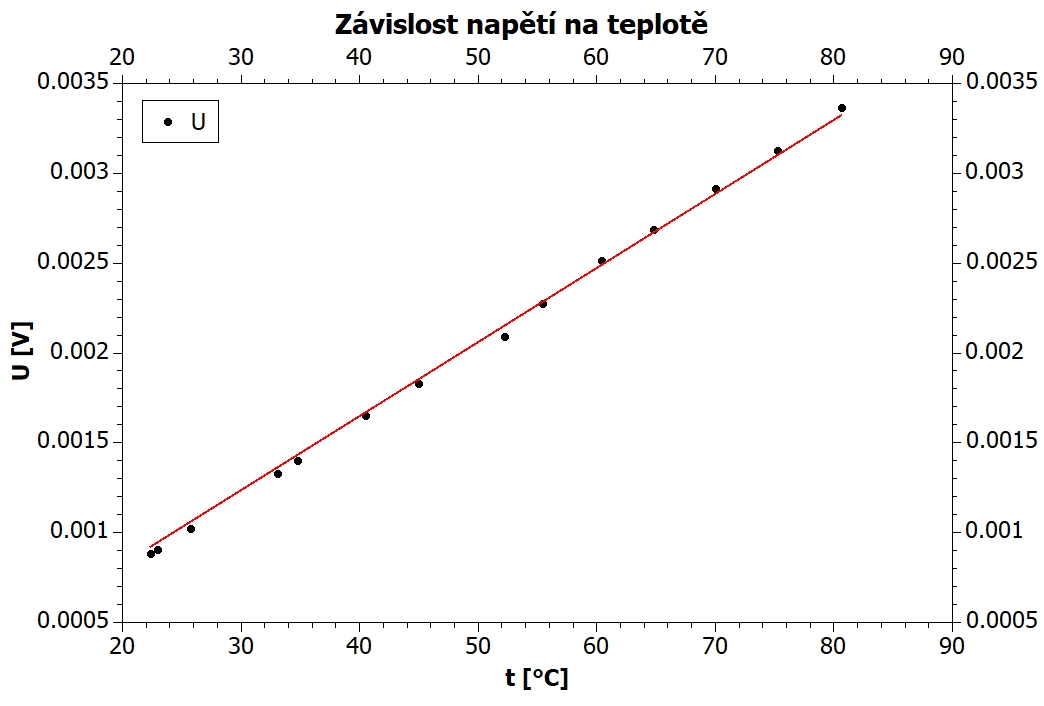
\includegraphics[width=1\linewidth, ]{napeti} 
			\caption{Graf závislosti napětí na teplotě s lineárními aproximacemi}
			\label{fig:subim1}
		\end{subfigure}
		\begin{subfigure}{0.4\textwidth}
			{\tiny \begin{verbatim}
					---------------------------------------------------------------------------------------
					[3/29/2024 1:12:18 AM	Plot: ''Graph2'']
					Linear Regression of dataset: Table1_U, using function: A*x
					Weighting Method: No weighting
					From x = 2.235000000000000e+01 to x = 8.059999999999999e+01
					A (slope) = 4.122027320386069e-05 +/- 1.732240671896891e-07
					--------------------------------------------------------------------------------------
					Chi^2/doF = 1.150788703342456e-09
					R^2 = 0.998362479968588
					Adjusted R^2 = 0.998226019965971
					RMSE (Root Mean Squared Error) = 3.39232767188321e-05
					RSS (Residual Sum of Squares) = 1.49602531434519e-08
					---------------------------------------------------------------------------------------
			\end{verbatim}}
			\caption{výsledky počítačové aproximace}
		\end{subfigure}
	\end{figure}
	
	V souladu s formulí (4) získáme Seebeckův koeficient:
	\begin{equation}
		\beta = 4.122 \cdot 10^{-5} \pm 0.017 \cdot 10^{-5} \, \text{V }. ^\circ \text{C}^{-1}
	\end{equation}
	Tato hodnota se nejvíce blíží termočlánku o složení chromel - alumel ($ 4.2 \cdot 10 ^{-5} \,\rm V . ^\circ C ^{-1}$), což je ostatně jedno z nejčastěji používaných čidel.\\
	\subsubsection{Druhá úloha}
	Získáváme následující grafy:
	\begin{figure}[H]
		
		\begin{subfigure}{0.6\textwidth}
			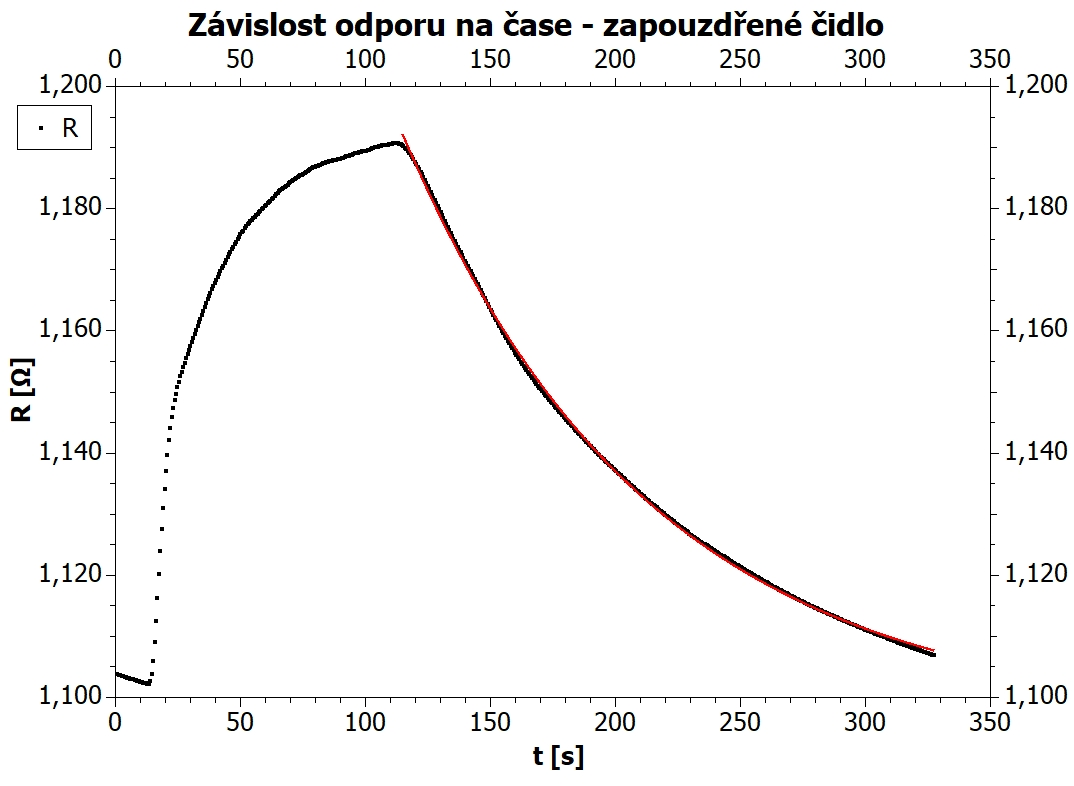
\includegraphics[width=1\linewidth, ]{zapouzdrene} 
			\caption{Graf závislosti odporu na čase}
			\label{fig:subim1}
		\end{subfigure}
		\begin{subfigure}{0.4\textwidth}
			{\tiny \begin{verbatim}
					[3/29/2024 2:22:02 AM	Plot: ''Graph6'']
					Exponential decay of dataset: Table3_R, using function: y0+A*exp(-x/t)
					Weighting Method: No weighting
					Scaled Levenberg-Marquardt algorithm with tolerance = 0.0001
					From x = 1.155260000000000e+02 to x = 3.271390600000000e+02
					A (amplitude) = 3.049424243569190e+02 +/- 1.235437953008848e+00
					t (e-folding time) = 9.910052453670433e+01 +/- 4.109632021518551e-01
					y0 (offset) = 1.096489714598173e+03 +/- 1.592473668725486e-01
					--------------------------------------------------------------------------------------
					Chi^2/doF = 2.183958822093816e-01
					R^2 = 0.999605591585544
					Adjusted R^2 = 0.999602367538559
					RMSE (Root Mean Squared Error) = 0.467328452171898
					RSS (Residual Sum of Squares) = 80.3696846530525
					---------------------------------------------------------------------------------------
					Iterations = 7
					Status = success
					---------------------------------------------------------------------------------------
			\end{verbatim}}
			\caption{výsledky exponenciálního fitu}
		\end{subfigure}
	\end{figure}
	Pro zapouzdřené čidlo získáváme 
	\begin{equation}
		\tau_m = 99.10 \pm 0.016 \,\rm s
	\end{equation}
	\begin{figure}[H]
		
		\begin{subfigure}{0.6\textwidth}
			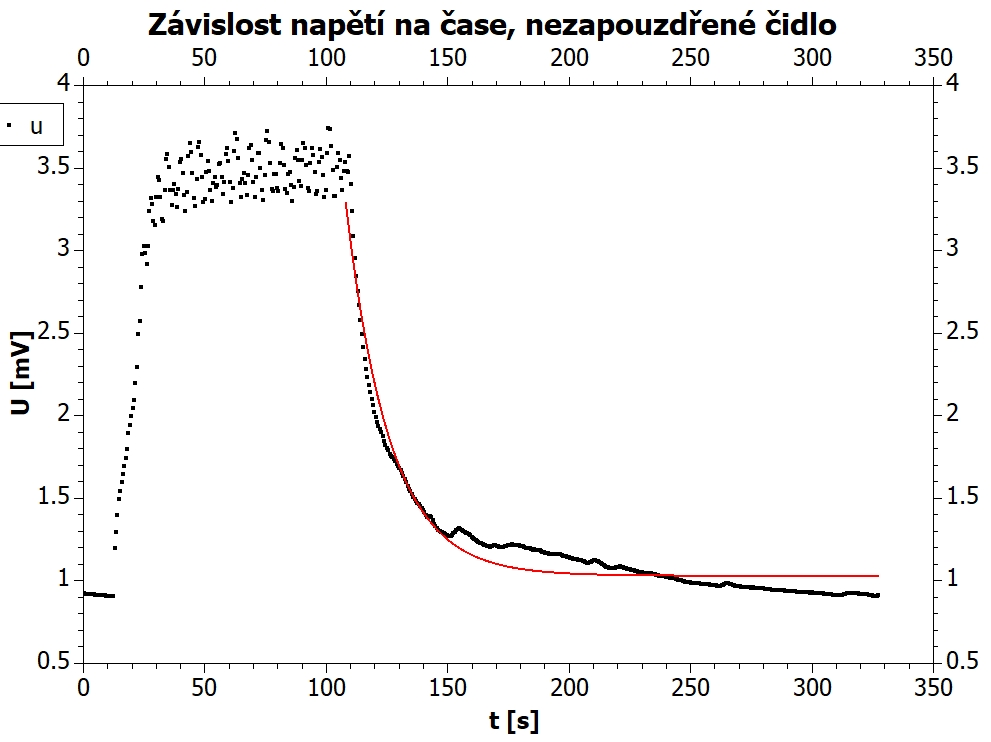
\includegraphics[width=1\linewidth, ]{nezapouzdrene} 
			\caption{Graf závislosti odporu na čase}
			\label{fig:subim1}
		\end{subfigure}
		\begin{subfigure}{0.4\textwidth}
			{\tiny \begin{verbatim}
					[3/29/2024 2:43:41 AM	Plot: ''Graph5'']
					Exponential decay of dataset: Table3_u , using function: y0+A*exp(-x/t)
					Weighting Method: No weighting
					Scaled Levenberg-Marquardt algorithm with tolerance = 0.0001
					From x = 1.0809384000000e+02 to x = 3.2713906000000e+02
					A (amplitude) = 9.1467769382112e+02 +/- 1.3878541710017e+02
					t (e-folding time) = 1.7982623758038e+01 +/- 4.2526289817182e-01
					y0 (offset) = 1.0316344449208e+00 +/- 5.9592369975803e-03
					--------------------------------------------------------------------------------------
					Chi^2/doF = 9.1711600854334e-03
					R^2 = 0.9512954976709
					Adjusted R^2 = 0.950910988442
					RMSE (Root Mean Squared Error) = 0.0957661740148
					RSS (Residual Sum of Squares) = 3.49421199255
					---------------------------------------------------------------------------------------
					Iterations = 26
					Status = success
					---------------------------------------------------------------------------------------
			\end{verbatim}}
			\caption{výsledky exponenciálního fitu}
		\end{subfigure}
	\end{figure}
	Pro nezapouzdřené čidlo získáváme 
	\begin{equation}
			\tau_m = 17.9 \pm 0.4 \,\rm s
	\end{equation}
	Můžeme si všimnout velkého rozdílu hodnot $\tau _m$ pro čidla. Výsledek, že relaxační doba bude pro nezapouzdřené čidlo významně kratší než pro čidlo zapouzdřené, je v souladu s našimi předpoklady. Právě pouzdro čidla zapříčiňuje akumulaci tepelné energie, čímž je přenos tepla mezi čidlem a okolím pomalejší. Čidlo s pouzdrem má mnohem větší tepelnou kapacitu než čidlo bez pouzdra - uvažujme n-krát větší hmotnost, a tím pádem i n-krát vyšší množství energie, které je v čidlu po dosažení cílové teploty uloženo, jehož následné předání zpět okolí trvá déle. Je nutné konstatovat, že relaxační doba $\tau_m$ značí pouze dobu, za kterou bude teplotní rozdíl aktuální a cílové teploty $e$-krát menší než rozdíl teploty cílové a počáteční.
	\subsection{měření teploty IR teploměrem}
	\subsubsection{První úloha}
		Získáváme následující údaje:\\ \\
	\begin{center}
			\begin{tabular}{l|lll|lll|lll}  
			& \multicolumn{3}{l}{Černá}       & \multicolumn{3}{l}{Lesklá}       & \multicolumn{3}{l}{Bílá}        \\ \hline
			& T [K]     & $T_p$ [K]  & $\varepsilon$ & T [K]       & $T_p$ [K]& $\varepsilon$ & T [K]     & $T_p$ [K]  & $\varepsilon$ \\ \hline
			1  & 561.02 & 562.55 & 1.011         & 560.88  & 424.75 & 0.329         & 560.74 & 561.85 & 1.008         \\ \hline
			2  & 560.20  & 557.95 & 0.984         & 558.72  & 421.65 & 0.324         & 557.24 & 556.85 & 0.997         \\ \hline
			3  & 556.45 & 553.65 & 0.980         & 553.79 & 414.85 & 0.315         & 551.12 & 552.35 & 1.009         \\ \hline
			4  & 550.02 & 548.65 & 0.990         & 549.74 & 416.35 & 0.329         & 549.45 & 546.75 & 0.980         \\ \hline
			5  & 548.82 & 546.95 & 0.986         & 547.79 & 415.25 & 0.330         & 546.75 & 542.85 & 0.972         \\ \hline
			6  & 545.40  & 539.05 & 0.954         & 543.03  & 405.15 & 0.310         & 540.66 & 536.75 & 0.971         \\ \hline
			7  & 539.61 & 536.15 & 0.975         & 538.26 & 405.75 & 0.323         & 536.9  & 533.25 & 0.973         \\ \hline
			8  & 536.20  & 534.55 & 0.988         & 534.73  & 400.95 & 0.316         & 533.26 & 530.25 & 0.978         \\ \hline
			9  & 532.10  & 524.15 & 0.942         & 532.03 & 400.05 & 0.320         & 531.95 & 521.15 & 0.921         \\ \hline
			10 & 520.12 & 519.85 & 0.998         & 519.88  & 397.35 & 0.341         & 519.64 & 513.85 & 0.956         \\ \hline
			&        &        &\textbf{ 0.981 }        &         &        & \textbf{0.324}         &        &        & \textbf{0.977}        
		\end{tabular}
	\end{center}
	Pro černou, lesklou a bílou část získáváme hodnoty emisivity: \\ $\varepsilon_{\text{Č}} = 0.981 \pm 0.007, \varepsilon_{\text{L}} = 0.324 \pm 0.003, \varepsilon_{\text{B}} = 0.977 \pm 0.009, (p = 0.6827, \nu = 9).$
	
	\subsubsection{Druhá úloha}
	\begin{center}
		\begin{tabular}{l|l|l|l}
		& $T_V$ [K]  & $T_O$ [K]  & $\tau$         \\ \hline
		Polykarbonát* & 467.15 & 297.65 & \textbf{0.0047} \\ \hline
		Sklo*         & 465.55 & 297.85 & \textbf{0.0052} \\ \hline
		SiO2*         & 456.65 & 297.95 & \textbf{0.0059} \\ \hline
		CaF2          & 455.45 & 400.65 & \textbf{0.5988} \\ \hline
		Ge            & 453.15 & 386.65 & \textbf{0.5300} \\ \hline
		KBr           & 450.45 & 440.35 & \textbf{0.9133} \\ \hline
		NaCl          & 448.25 & 425.05 & \textbf{0.8085} \\ \hline
		PE500         & 446.65 & 308.75 & \textbf{0.2283} \\ \hline
		Si            & 444.65 & 388.85 & \textbf{0.5849} \\ \hline
		GaAs          & 443.45 & 394.35 & \textbf{0.6254} \\ \hline
		Cu*           & 441.55 & 297.25 & \textbf{0.0048}
	\end{tabular}
	\end{center}
	Pro získání propustnosti jsme aplikovali formule (8) a (9), druhá formule byla aplikována pro látky označené *.
	\subsubsection{Třetí úloha}
	Po odborné aplikaci námrazy na vychlazenou měděnou desku dýchnutím byly změřeny teploty \,\,\, \,\,\,\,\,\,\, $T$~-~kontaktním teploměrem - a $T_p$ - IR teploměrem. Měření bylo opakováno po odstranění námrazy žiletkou. Získali jsme následující údaje o emisivitě:
\begin{center}
		\begin{tabular}{l|l|l|l}
		& T [K]  & $T_p$ [K] & $\varepsilon$ \\ \hline
		S námrazou  & 255.35 & 261.85    & 1.110         \\\hline
		Bez námrazy & 256.65 & 295.95    & 1.768       
	\end{tabular}
\end{center}
	Vidíme, že jsme dosáhli nereálného výsledku - emisivita z podstaty definice \textbf{nemůže} být vyšší než jedna. Systematická chyba je v tomto případě způsobena odraženým zářením. Teplota získaná IR teploměrem je vyšší než teplota skutečná, jelikož teploměr měří i okolní záření objektů pokojové teploty. Toto záření se pokusíme eliminovat položením vychlazené kovové hemisféry s otvorem na destičku a měřením skrze otvor. Teplota je však stále vyšší, než teplota měřená kontaktním teploměrem ($T_p = 272.15$ K), znovu bychom získali emisivitu nereálné hodnoty. V tomto případě chyba nejspíše pramení v záření samotného teploměru, které se mezi deskou a hemisférickou slupkou odráží zpět do měřícího přístroje.

	
	\section{Závěr}
	U čidel se nám úspěšně podařilo změřit závislosti odporu, resp. napětí na teplotě a určit, o jaký typ se jednalo. Měření relaxační doby nám ukázalo, že zapouzdřené čidlo na změny teplot reaguje pomaleji. Měření IR teploměrem ukázalo, že AČR se těleso může blížit nezávisle na barvě povrchu, reflexní vrstvy emisivitu však snižují. Podařilo se nám změřit propustnost deseti různých povrchů a~změřili jsme zdánlivé teploty vychlazené měděné desky, u této úlohy se nám však nepodařilo eliminovat odražené okolní záření a úspěšně změřit emisivitu.

	
	% Nakonec nezapomeňte projet text programem vlna nebo vlnka, např.
	% 	vlna -m -l -n mojeuloha.tex
	% nebo zkontrolovat a opravit jednopísmenné předložky na koncích řádků ručně.
	
	
\end{document}
